\documentclass{standalone}
\usepackage{tikz}
\usepackage{ctex,siunitx}
\usepackage{tkz-euclide}
\usepackage{amsmath}
\usetikzlibrary{patterns, calc}
\usetikzlibrary {decorations.pathmorphing, decorations.pathreplacing, decorations.shapes,}
\begin{document}
\small
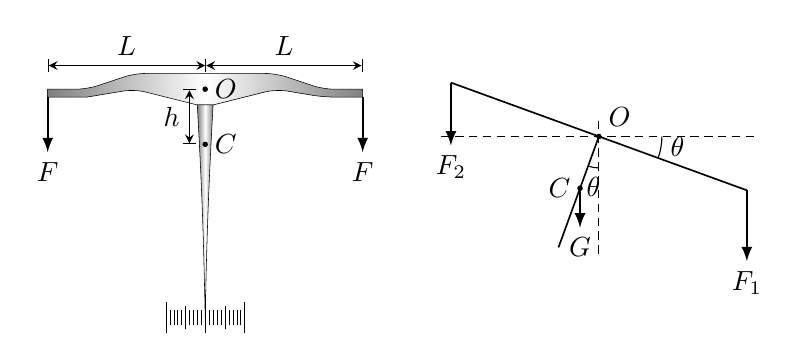
\begin{tikzpicture}[>=stealth,scale=1.0]
  \draw[very thin,left color=gray,right color=gray,middle color=white](-2,-0.2)--++(0,0.1)[rounded corners]--++(0.5,0)--++(0.6,0.2)--++(1.8,0)--++(0.6,-0.2)[sharp corners]--++(0.5,0)--++(0,-0.1)[rounded corners]--++(-0.5,0)--++(-0.6,0.1)[sharp corners]--++(-0.8,-0.2)--++(-0.2,0)[rounded corners]--++(-0.8,0.2)[sharp corners]--++(-0.6,-0.1)--cycle;
  \draw[very thin,left color=gray,right color=gray,middle color=white] (-0.1,-0.3)to[bend left=1](0,-3)to[bend left=1](0.1,-0.3)--cycle;
  \foreach \x in{1,2,3,4,6,7,8,9}
  {
    \draw[ultra thin] (0.05*\x,-3.1)--++(0,0.2);
    \draw[ultra thin] (-0.05*\x,-3.1)--++(0,0.2);
  }
  \foreach \x in {5,-5}
  {\draw[ultra thin] (0.05*\x,-3.15)--++(0,0.3);}
  \foreach \x in {10,-10,0}
  {\draw[ultra thin] (0.05*\x,-3.2)--++(0,0.4);}
  \fill(0,-0.8)circle(1pt)node[right]{$C$};
  \fill(0,-0.1)circle(1pt)node[right]{$O$};
  \draw[thin,|<->|](-0.2,-0.8)--(-0.2,-0.1)node[midway,left]{$h$};
  \draw[thin,|<->](-2,0.2)--(0,0.2)node[midway,above]{$L$};
  \draw[thin,|<->|](0,0.2)--(2,0.2)node[midway,above]{$L$};
  \draw[thick,-latex](-2,-0.2)--++(0,-0.7)node[below]{$F$};
  \draw[thick,-latex](2,-0.2)--++(0,-0.7)node[below]{$F$};
  \begin{scope}[xshift=5cm,yshift=-0.7cm]
    \draw[densely dashed](-2,0)--(2,0)(0,0.2)--(0,-1.5);
    \fill(250:0.7)circle(1pt)node[left]{$C$};
    \fill(0,0)circle(1pt)node[above right]{$O$};
    \draw[semithick](160:2)--(-20:2)(0,0)--(250:1.5);
    \draw[thick,-latex](250:0.7)--++(0,-0.5)node[below]{$G$};
    \draw[thick,-latex](160:2)--++(0,-0.8)node[below]{$F_2$};
    \draw[thick,-latex](-20:2)--++(0,-0.9)node[below]{$F_1$};
    \draw[thin](0,-0.4)arc(270:250:0.4)node[midway,below]{$\theta$};
    \draw[thin](0.8,0)arc(0:-20:0.8)node[midway,right]{$\theta$};
  \end{scope}
\end{tikzpicture}
\end{document}